%%%%%%%%%%%%%%%%%%%%%%%%%%%%%%%%%%%%%%%%%%%%%%%%%%%%%%%%%%%%%%%%%%%%%%%%
%%%%%                                                              %%%%%
%%%%% Chapter 2: Background                                        %%%%%
%%%%%                                                              %%%%%
%%%%%%%%%%%%%%%%%%%%%%%%%%%%%%%%%%%%%%%%%%%%%%%%%%%%%%%%%%%%%%%%%%%%%%%%
\chapter{Background}
\label{ch2}

%%%%%%%%%%%%%%%%%%%%%%%%%%%%%%%%%%%%%%%%%%%%%%%%%%%%%%%%%%%%%%%%%%%%%%%%
%%%%%%%%%%%%%%%%%%%%%%%%%%%%%%%%%%%%%%%%%%%%%%%%%%%%%%%%%%%%%%%%%%%%%%%%
%%%%%%%%%%%%%%%%%%%%%%%%%%%%%%%%%%%%%%%%%%%%%%%%%%%%%%%%%%%%%%%%%%%%%%%%
\section{Nanopore sequencing}
%% Intro

%%% History of nanopore development
\paragraph{A brief history of nanopore sequencing}
%% Initial idea and expreiments
The concept of nanopore sequencing is based on the idea that as a
single-stranded DNA (or RNA) translocates through a nanometer sized
pore, a nanopore, in the presence of an electric field, the change in
current level measured across the nanopore would be dependent on the
nucleotide passing through the nanopore; Thus, measuring the current
over time could be leveraged to determine the sequence of nucleotides
(Fig.~\ref{nanopore}b).
%
This idea of using transmemberane proteins an nanopores for sensing and
sequencing nucleic acids was independently thought of by several
researches including David Deamer, Hagan Bayley, and George Church
\citep{deamer2016three,bayley2015nanopore,branton2010potential}.

%% Initial expreiments
% Detecting the presence of oligos
Initial experiments showed that as a single-stranded DNA or RNA
molecules could be driven through a \emph{Staphylococcus aureus}
$\alpha$-hemolysin in the presence of an electric field
\citep{kasianowicz1996characterization}. The current through the pore
remained constant in the absence of oligomers; and the presence of oligomers
caused transient decreases in current, with the duration of the decrease
proportional to the length of the oligomer.
% Detecting the bases in oligos
Further research demonstrated that decrease in amplitude of current
could be used to differentiate between poly-purine and poly-pyrimidine
sequences of RNA \citep{akeson1999microsecond} and DNA
\citep{meller2000rapid}. It was also observed that the DNA molecules
translocate through the nanopore at few microseconds per base
\citep{meller2000rapid}.

\begin{figure}[b!]
\centering
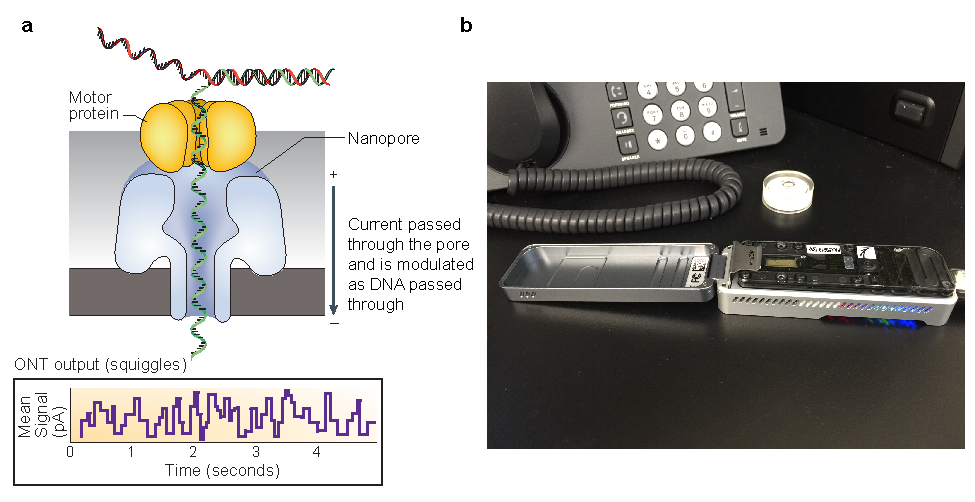
\includegraphics{nanopore.pdf}
\caption{Nanopore sequencing. (a) Current across a nanopore is
  measured as a DNA molecule translocates through a nanopore. This figure is
  adapted from Figure 5Ab in \cite{goodwin2016coming}. (b) Oxford Nanopore
  Technologies MinION instrument.}
\label{nanopore}
\end{figure}

%% Challenges for sequencing DNA
Although these experiments demonstrated the potential for nanopores to
distinguish nucleic acid polymers, several challenges remained to be
addressed to use this approach for reading individual bases on a DNA or
RNA molecule.
%
The most important of these were detecting the bases on a molecule at
single nucleotide resolution and slowing the rate of translocation
through the nanopore so that a readout can be obtained
\citep{bayley2015nanopore,branton2010potential}.
%
These challenges were resolved in the forthcoming years. A few
notable milestones are described below.

%% Single nucleotide detection
In regard to identifying individual nucleobases, all four bases were
identified in single-stranded DNA that have a terminal hairpin structure
\citep{ashkenasy2005recognizing} and single-stranded DNA attached to
streptavidin with a biotin linker
\citep{purnell2009discrimination,stoddart2009single}. These structures
immobilized the DNA in the nanopore (either a wildtype
$\alpha$-hemolysin or an engineered form of it) allowing sufficient time
for detection. Thus, with the appropriate sequence, each base could be
resolved, and further, the location within a nanopore that is most
sensitive to detect bases was also determined.


%% engineered nanopores
The frequency of translocation of DNA molecules through a
$\alpha$-hemolysin pore was increased and the voltage threshold for
translocation was decreased by engineering the pore to have positive
charged groups in the lining of the lumen \citep{maglia2008enhanced}.
%
However, a disadvantage of the $\alpha$-hemolysin pores is that the
region that is sensitive to the nucleotides in the pore is too wide, and
so the current differences are small between nucleotides, making single
nucleotide detection difficult.
%
Pores derived from \emph{Mycobacterium smegmatis} porin A has a narrower
sensitive region, and could detect nucleotides at a higher resolution
\citep{butler2008single,manrao2011nucleotide}.

%% processivity control
In regard to controlling the rate of translocation through a nanopore,
there were two approaches, exo-sequencing and strand-sequencing.
% exo-sequencing
In the exo-sequencing approach, individual bases from a DNA are cleaved
into a nanopore with an exonuclease and unidentified one at a time
\citep{astier2006toward,clarke2009continuous}.
% strand-sequencing
Alternatively, in the strand sequencing approach a DNA molecule is
threaded though a nanopore at a controlled rate and the bases are
identified from the continuous change in current levels. Initial
approaches in strand sequencing used a DNA polymerase (derived from
\emph{Escherichia coli} Kleenow fragment or bacteriophage T7) and
recorded the current levels as the DNA translocates through a pore with
the incorporation of each nucleotide
\citep{benner2007sequence,cockroft2008single,gyarfas2009mapping,
chu2010real}.
%
Subsequently it was shown that $\phi$29 polymerase could be used to control
ratcheting in both the forward and the reverse direction
\citep{lieberman2010processive,manrao2012reading,cherf2012automated}.
$\phi$29 was used to sequence reads up to 4.5 kb from the $\phi$X174 genome
using nanopores \citep{laszlo2014decoding}.


%% Oxford nanopore technologies
\paragraph{Oxford Nanopore Technologies}
Oxford Nanopore Technologies was founded in 2005 by Hagan Bayley and
colleagues \citep{deamer2016three}. Oxford Nanopore Technologies
announced the MinION instrument at the Advances in Genome Biology and
Technology meeting in 2012 and made it available to early access
researches in 2014 \citep{deamer2016three,bayley2015nanopore}.

%% Oxford MinION
The MinION sequencer (Fig.~\ref{nanopore}b) is a portable instrument
requiring just a modest computer for control and data acquisition.  A
MinION flowcell of 2048 nanopores (at present, a derivative of
\emph{Escherichia coli} CsgG protein \citep{brown2016nanopore}) embedded
on a membrane, of which 512 pores can sequence molecules in parallel.

%% Current state of nanopore sequencing
Whole genomes of several organisms including humans have been sequenced
using the MinION instrument \citep{loman2015complete,stancu2017mapping,
jain2018nanopore,bowden2019sequencing,moss2020complete}. It has also
been used in several other applications such as disease surveillance
\citep{quick2016real,faria2016mobile}, metagenomics
\citep{goordial2017situ,charalampous2019nanopore,leggett2020rapid},
direct RNA sequencing \citep{garalde2018highly,workman2019nanopore,
depledge2019direct}, and detecting methylated bases
\citep{rand2017mapping,simpson2017detecting,liu2019accurate} among
others \citep{jain2016oxford}.

%% other decives from ONT
In addition to the MinION instrument, Oxford Nanopore Technologies
currently offers various nanopore devices including the bench-top
GridION and PromethION which allows parallel sequencing with up to 5 and
48 flowcells, respectively.


%% Nanopore library construction
\paragraph{Nanopore library preparation and sequencing}
%% TODO: is it called library preparation or sample preparation
Sequencing nucleic acids requires prepossessing the sample DNA for
compatibility with the underlying sequencing technology, a process
traditionally referred to as library preparation.
%
Sequencing on a nanopore machine usually requires fragmenting DNA
molecules to the appropriate length and attaching sequencing adapters.
%
Oxford nanopore technologies offers several commercially library
preparation kits for both DNA and RNA samples.  The most frequently used
of these kits are the Ligation Sequencing Kit family and the Rapid
Sequencing Kit family.

% Ligation kit
In theory, there is no limit on the length of a molecule that can be
sequenced with a nanopore, and thus, the length is determined by the
downstream application or the limitations of handling high molecular
weight DNA. For the ligation sequencing kit (SQK-LSK108 1D DNA by
ligation), the recommended length is
$\sim$8 kb when starting with 1ug of sample to ensure appropriate molar
concentration in the subsequent steps.  DNA molecules can be fragmented
to the appropriate length using a variety of methods including the
Covaris g-TUBE.
%
These molecules are then optionally repaired to remove any nicks, and
then the DNA ends are prepared to have a dA tail. Finally, sequencing
adapters (that have a dT tail) are ligated to the end-prepared DNA.
These adapters contain specific DNA sequenced with attached enzymes
that regulate translocation of the DNA molecule into a nanopore.
Library preparation with the ligation kit takes approximately 60 minutes.

% Rapid kit
The rapid library preparation kit (SQK-RAD003 Rapid sequencing) offers a
faster method, by simultaneously fragmenting and tagging the ends of
high molecular weight DNA (recommended $>$ 30 kb). Adapters are then
attached to these tags.  Library preparation with the rapid kit takes
approximately 10 minutes.

% Barcoding capablities
Both of these kits offer barcoding capabilities for multiplexing several
samples in a single sequencing run. For example, the Native Barcode Kit
(EXP-NBD103) is used in addition to the ligation sequencing kit, and
adds a barcode sequence to the end-prepared DNA molecules prior to
ligating sequencing adapters. After library preparation with a unique
barcode for each sample, they can pooled in appropriate molar
concentrations before sequencing.

% Brief summary of other kits
Oxford Nanopore Technologies offers severs other preparation kits, such
as the $\text{1D}^2$ kit for higher accuracy reads and PCR based kits when
starting with nanogram or picogram amounts of DNA.

% After lib. prep.: loading and sequencing
After library construction the sample is ready to be sequenced. The
flowcell is loaded on the sequencing machine, primed with the appropriate
buffers, and the sample is loaded. After which the sequencing can be
started and the reads are available as they are sequenced in real-time.
%
The sequencing process is controlled by the MinKNOW tool, and can
continue for up to 48 hours.
% Base-calling reads
The sequenced reads can either be base-called in real time using the
MinKNOW or at a later time using the Guppy tool.

%% Properties of nanopore reads
\paragraph{Properties of nanopore reads}



%%%%%%%%%%%%%%%%%%%%%%%%%%%%%%%%%%%%%%%%%%%%%%%%%%%%%%%%%%%%%%%%%%%%%%%%
%%%%%%%%%%%%%%%%%%%%%%%%%%%%%%%%%%%%%%%%%%%%%%%%%%%%%%%%%%%%%%%%%%%%%%%%
%%%%%%%%%%%%%%%%%%%%%%%%%%%%%%%%%%%%%%%%%%%%%%%%%%%%%%%%%%%%%%%%%%%%%%%%
\section{Copy number variation and profiling}


%%%%%%%%%%%%%%%%%%%%%%%%%%%%%%%%%%%%%%%%%%%%%%%%%%%%%%%%%%%%%%%%%%%%%%%%
%%%%%%%%%%%%%%%%%%%%%%%%%%%%%%%%%%%%%%%%%%%%%%%%%%%%%%%%%%%%%%%%%%%%%%%%
%%%%%%%%%%%%%%%%%%%%%%%%%%%%%%%%%%%%%%%%%%%%%%%%%%%%%%%%%%%%%%%%%%%%%%%%
\section{Prior protocols based on concatenating DNA molecules}
%%% SAGE
\paragraph{Serial analysis of gene expression (SAGE)}
The concept of ligating short DNA molecules to improve the efficiency
of sequencing was introduced in serial analysis of gene expression
(SAGE) \citep{}, and subsequently its variants such as LongSAGE and
SuperSAGE \citep{}. SAGE

%%% variants of SAGE
\paragraph{Variants of SAGE}

% Digital karyotyping
\paragraph{Digital karyotyping}

% SMASH
\paragraph{SMASH}

% concat-seq
\paragraph{Concat-seq}

